% MCM/ICM 2026 LaTeX 主控文件
% 编译:XeLaTeX + Biber
% !TEX program = xelatex
% !BIB program = biber

\documentclass{mcmthesis}

% --- 兼容性补丁 ---
% 避免旧的 .aux/.toc 中残留的 \thechapter(常见于曾启用 algochapter 时)导致 hyperref 报错
\newcounter{chapter}
\renewcommand{\thechapter}{\arabic{chapter}}

% --- MCM 题目配置 ---
% 【重要】比赛时务必修改 tcn 为你的真实队伍编号
\mcmsetup{
    tcn = {2617892},        % Team Control Number(队伍编号)
    problem = {C},          % 选择的题目 (A/B/C/D/E/F)
    sheet = true,           % 生成官方 Summary Sheet(摘要首页)
    titleinsheet = true,    % 在 Summary Sheet 上显示标题
    keywordsinsheet = true, % 在 Summary Sheet 上显示关键词
    titlepage = false       % 禁用独立标题页,防止摘要重复
}

% 目录开关:若模板提供 \showtoctrue,则显式开启
\makeatletter
\@ifundefined{showtoctrue}{}{\showtoctrue}
\makeatother

% 宏包加载区

% --- 字体与排版 ---
\usepackage{palatino}
\usepackage{microtype}
\setlength{\emergencystretch}{2em}
% \usepackage{lipsum}             % 占位文字(已移除,避免占位文本进入终稿)

% --- 页面与布局 ---
\usepackage{lastpage}           % 获取总页数
\usepackage{zref-abspage}       % 获取物理页码(避免 \maketitle 等重置 page 计数器)
\usepackage{float}              % 强制图表位置 [H] 选项
\usepackage{geometry}           % 页边距微调(如需)
\setlength{\headheight}{15pt}   % 修复 fancyhdr 警告

% --- 数学公式 ---
\usepackage{amsmath, amssymb, amsthm}  % AMS 数学三件套
\usepackage{mathtools}          % amsmath 增强版

% --- 表格美化(核心!)---
\usepackage{booktabs}           % 【必须】三线表:\toprule, \midrule, \bottomrule
\usepackage{tabularx}           % 【必须】自动列宽表格,支持长文本换行
\usepackage{longtable}          % 跨页长表格
\usepackage{multirow}           % 表格单元格合并
\usepackage{array}              % 表格列格式增强

% --- 算法与伪代码(顶会风格)---
% 【重要】使用 ruled + vlined + linesnumbered 呈现计算机顶会论文风格
% 说明:mcmthesis 为 article 体裁,没有 chapter 计数器,需移除 algochapter 选项
\usepackage[ruled, vlined, linesnumbered]{algorithm2e}
\SetAlgorithmName{Algorithm}{algorithm}{List of Algorithms}
\SetKwInput{KwIn}{Input}        % 输入
\SetKwInput{KwOut}{Output}      % 输出
\SetKwInput{KwData}{Data}       % 数据
\SetKwInput{KwResult}{Result}   % 结果

% --- 代码高亮 ---
\usepackage{listings}
\lstset{
    basicstyle=\small\ttfamily,
    keywordstyle=\color{blue},
    commentstyle=\color{gray},
    numbers=left,
    numberstyle=\tiny\color{gray},
    frame=single,
    breaklines=true,
    tabsize=4
}

% --- 图形与颜色 ---
\usepackage{graphicx}           % 插入图片
\usepackage{subcaption}         % 子图
\usepackage{xcolor}             % 颜色支持
\usepackage{tikz}               % 绘图(流程图等)
\usetikzlibrary{shapes, arrows, positioning, calc}

% --- 列表与枚举 ---
\usepackage{enumitem}           % 自定义列表样式
\setlist[enumerate]{itemsep=0pt, parsep=0pt}  % 紧凑列表

% --- 超链接(放在最后加载)---
\usepackage{hyperref}
\hypersetup{
    colorlinks=true,
    linkcolor=blue!70!black,
    citecolor=green!50!black,
    urlcolor=blue!80!black
}

% --- 参考文献配置 ---
% 【提示】可根据需要切换为 IEEE 风格: style=ieee
\usepackage[backend=biber, style=ieee, sorting=none]{biblatex}
\addbibresource{ref.bib}

% 自定义计数器与命令

% --- 正文页数计数器(实现 "Page X of Y" 功能)---
\newcounter{mainpages}          % 保存正文总页数

% 写入 aux 文件的命令
\makeatletter
\newcommand{\savemainpages}{%
    \immediate\write\@auxout{\string\setcounter{mainpages}{\the\value{page}}}%
}

\makeatother

% --- 自定义引用命令 ---
\newcommand{\figref}[1]{Fig.~\ref{#1}}      % 图引用
\newcommand{\tabref}[1]{Table~\ref{#1}}     % 表引用
\newcommand{\eqnref}[1]{Eq.~(\ref{#1})}     % 公式引用
\newcommand{\algref}[1]{Algorithm~\ref{#1}} % 算法引用
\newcommand{\secref}[1]{Section~\ref{#1}}   % 章节引用

% 文档元信息

\title{A Data-Driven Multi-Objective Optimization Framework for \\
       Sustainable Resource Allocation: An MCM 2026 Approach}
\author{Team \#2617892}

% 正文开始
\begin{document}

% 页码策略:从 Summary 起连续计数;Summary/目录隐藏页码但计入总页数
\pagenumbering{arabic}
\setcounter{page}{1}

% PART 0: 摘要页
% 【说明】mcmthesis 的 \maketitle 会自动生成官方 Summary Sheet
% 摘要内容在 sections/00_abstract.tex 中定义
% Summary Sheet:隐藏页码但保留计数
\pagestyle{empty}
\begin{abstract}%以下是25年C题的参考Abstract
    
To ensure a systematic and multidimensional approach to Olympic medal prediction, this study constructs a dynamic and coupled comprehensive \textbf{Predictive Framework}. This framework integrates various objectives, including medal distribution prediction, breakthrough country identification, event performance evaluation, and the impact analysis of coaching resource allocation. By employing multi-source heterogeneous data fusion and machine learning integration methods, we achieve an in-depth analysis and reliable prediction of the development patterns in competitive sports.

First, we develop a multidimensional predictive model to analyze Olympic medal patterns. Utilizing \textbf{Principal Component Analysis (PCA)} for dimensionality reduction and noise filtering of the Olympic event dataset, we combine \textbf{Long Short-Term Memory (LSTM)} networks to mine temporal features and integrate home advantage effects. A dual-channel \textbf{XGBoost-Bootstrap} model is established to generate predictions with a 95\% confidence interval. The results indicate an upward trend for countries such as the United States and the United Kingdom, while countries like France and China show a decline. The model exhibites a high accuracy with a low \textbf{MAE} and \textbf{MAPE}, demonstrating strong robustness. Through non-parametric testing, potential breakthrough countries are identified, with San Marino and Kuwait showing gold medal breakthrough probabilities of \textbf{84.7\%} and \textbf{68.4\%}, respectively.

Subsequently, we develop a \textbf{Difference-in-Differences (DID)} model to quantify the competitive benefits of coaching replacement and conduct statistical significance tests as well as parallel trends tests to ensure the reliability of our results. It is found that during the 2020-2024 period, Australia, South Korea, and Poland experienced significant "great coach" policy effects through strategic restructuring of their coaching teams. Based on this, we recommend prioritizing investment in high-elasticity projects. \textbf{SHapley Additive exPlanations (SHAP)} is further utilized to quantify event contributions, revealing that swimming and athletics serve as core contributing events to medal augmentation.

Furthermore, we explore the potential of a country to win its first-ever medal by constructing a \textbf{Hurdle-Tobit} fusion model. This model addresses the zero-inflation characteristics and heterogeneity between countries. The prediction results show that countries like Angola and Bangladesh have a probability of winning their first medal exceeding \textbf{45\%} in the next Games. Finally, we propose a strategic resource allocation plan using \textbf{Multiobjective Optimization} to balance the "depth" and "breadth" of National Olympic Committees (NOCs), suggesting that high-potential NOCs should prioritize multinational coach introductions in wrestling and table tennis.

In conclusion, our integrated framework synthesizes all models and analyses to present new insights and corresponding decision supports for the global sports community.

\begin{keywords}
    Olympic Medal Prediction, PCA-LSTM, XGBoost, DID Model, Hurdle-Tobit, SHAP Analysis.
\end{keywords}

\end{abstract}

\maketitle
\thispagestyle{empty}

% PART 1: 目录页
% 【重要】目录页使用罗马数字编号 (i, ii, ...),不计入 25 页限制
\newpage
\pagestyle{empty}
\tableofcontents
\thispagestyle{empty}

% PART 2: 正文
% 【重要】正文从阿拉伯数字 1 开始,显示 "Page X of Y"
\newpage
\setcounter{page}{\numexpr\value{abspage}+1\relax}
\pagestyle{fancy}
\fancyhf{} % 清空页眉页脚
\fancyhead[L]{\small Team \#2617892}
\fancyhead[R]{\small Page \thepage\ of \themainpages}
\fancyfoot[C]{} % 页脚留空

% --- 正文各章节 ---
% Section 1: Introduction
% 引言:问题背景 + 问题重述 + 利益相关者 + 本文工作

\section{Introduction}
\label{sec:intro}

%=== 1.1 问题背景:强调可持续性挑战 ===
\subsection{Problem Background}
\label{subsec:background}

% 【写作指导】E题引言需强调:
% 1. 环境问题的紧迫性与全球性
% 2. 多利益相关者的复杂博弈
% 3. 可持续发展的长期视角

The 21st century confronts humanity with unprecedented environmental challenges that demand integrated, systems-oriented solutions. \TODO{Describe the specific environmental context of Problem E, e.g., ecosystem degradation, climate adaptation, resource scarcity, clean energy transition.}

The complexity of this challenge arises from several intertwined factors:

\begin{itemize}[itemsep=0.3em]
    \item \textbf{Interconnected Systems:} Environmental, economic, and social systems are deeply coupled, with interventions in one domain producing cascading effects across others.
    
    \item \textbf{Temporal Dynamics:} Sustainability outcomes unfold over decades, requiring models that capture both short-term trade-offs and long-term equilibria.
    
    \item \textbf{Stakeholder Heterogeneity:} Different actors---governments, industries, communities, and future generations---hold divergent values and objectives that must be reconciled.
    
    \item \textbf{Deep Uncertainty:} Climate variability, technological disruptions, and policy shifts introduce substantial uncertainty into any planning framework.
\end{itemize}

\TODO{Add 1-2 paragraphs with specific statistics and references relevant to the Problem E topic. Cite authoritative sources such as IPCC, UN SDGs, or peer-reviewed literature.}

%=== 1.2 问题重述:精确界定任务 ===
\subsection{Restatement of the Problem}
\label{subsec:restatement}

To address the requirements of the 2026 ICM Problem E, we are tasked with developing a comprehensive analytical framework to:

\begin{enumerate}[itemsep=0.4em]
    \item \textbf{Task 1: \TODO{First Sub-Problem}}
    
    \TODO{Restate the first specific question from Problem E. Example: ``Develop a sustainability indicator system that captures environmental, economic, and social dimensions of [topic].''}
    
    \item \textbf{Task 2: \TODO{Second Sub-Problem}}
    
    \TODO{Restate the second specific question. Example: ``Model the dynamic interactions between [key system components] over a [time horizon].''}
    
    \item \textbf{Task 3: \TODO{Third Sub-Problem}}
    
    \TODO{Restate the third specific question. Example: ``Evaluate alternative policy scenarios and identify optimal intervention strategies.''}
    
    \item \textbf{Task 4: \TODO{Fourth Sub-Problem / Policy Memo}}
    
    \TODO{Restate the policy communication requirement. Example: ``Prepare a concise policy brief for [target decision-maker] summarizing key findings and recommendations.''}
\end{enumerate}

%=== 1.3 利益相关者与目标分析 ===
\subsection{Stakeholders and Objectives}
\label{subsec:stakeholders}

% 【E题核心】利益相关者分析是O奖论文的标志性要素
A sustainability-oriented decision framework must explicitly acknowledge the diverse stakeholders affected by and influencing the system. Table~\ref{tab:stakeholders} maps key stakeholders to their primary objectives and potential conflicts.

\begin{table}[H]
    \centering
    \caption{Stakeholder Analysis Matrix}
    \label{tab:stakeholders}
    \begin{tabularx}{\textwidth}{l X X X}
        \toprule
        \textbf{Stakeholder} & \textbf{Primary Objectives} & \textbf{Constraints} & \textbf{Potential Conflicts} \\
        \midrule
        \TODO{Government} & 
        \TODO{Environmental protection, economic growth, public welfare} & 
        \TODO{Budget limitations, political cycles} & 
        \TODO{Short-term growth vs. long-term sustainability} \\
        \addlinespace[0.5em]
        
        \TODO{Communities} & 
        \TODO{Livelihoods, health, cultural preservation} & 
        \TODO{Limited resources, information asymmetry} & 
        \TODO{Development vs. conservation} \\
        \addlinespace[0.5em]
        
        \TODO{Private Sector} & 
        \TODO{Profitability, market share, compliance} & 
        \TODO{Competition, capital constraints} & 
        \TODO{Cost externalization vs. responsibility} \\
        \addlinespace[0.5em]
        
        \TODO{NGOs} & 
        \TODO{Advocacy, transparency, equity} & 
        \TODO{Funding, influence} & 
        \TODO{Radical vs. incremental change} \\
        \addlinespace[0.5em]
        
        \TODO{Future Gen.} & 
        \TODO{Intergenerational equity, resources} & 
        \TODO{No direct voice} & 
        \TODO{Present vs. future well-being} \\
        \bottomrule
    \end{tabularx}
\end{table}

% 目标层次结构
Our framework adopts a \textbf{hierarchical objective structure} aligned with the three pillars of sustainability:

\begin{enumerate}[itemsep=0.2em]
    \item \textbf{Environmental Pillar:} \TODO{e.g., Minimize carbon emissions, preserve biodiversity, maintain ecosystem services}
    \item \textbf{Economic Pillar:} \TODO{e.g., Maximize cost-effectiveness, ensure economic viability, create green jobs}
    \item \textbf{Social Pillar:} \TODO{e.g., Promote equitable distribution, protect vulnerable populations, enhance quality of life}
\end{enumerate}

%=== 1.4 本文工作概述 ===
\subsection{Our Work}
\label{subsec:ourwork}

Our study introduces a \textbf{sustainability-oriented decision support framework} with the following methodological contributions:

\begin{enumerate}[itemsep=0.4em]
    \item \textbf{Three-Pillar Indicator System:}
    A comprehensive sustainability assessment framework integrating environmental, economic, and social dimensions through AHP-Entropy hybrid weighting.
    
    \item \textbf{System Dynamics Modeling:}
    A feedback-driven model capturing nonlinear interactions, tipping points, and long-term system trajectories under different policy regimes.
    
    \item \textbf{Scenario-Based Analysis:}
    Four carefully designed scenarios (BAU, Moderate, Aggressive, Stress Test) that span the policy option space and stress-test system resilience.
    
    \item \textbf{Multi-Criteria Decision Analysis:}
    TOPSIS-based ranking complemented by explicit trade-off frontier visualization to support transparent decision-making.
    
    \item \textbf{Actionable Policy Recommendations:}
    Tiered, stakeholder-specific recommendations with implementation roadmaps and adaptive management provisions.
\end{enumerate}

% 【插入框架流程图占位符】
\begin{figure}[H]
    \centering
    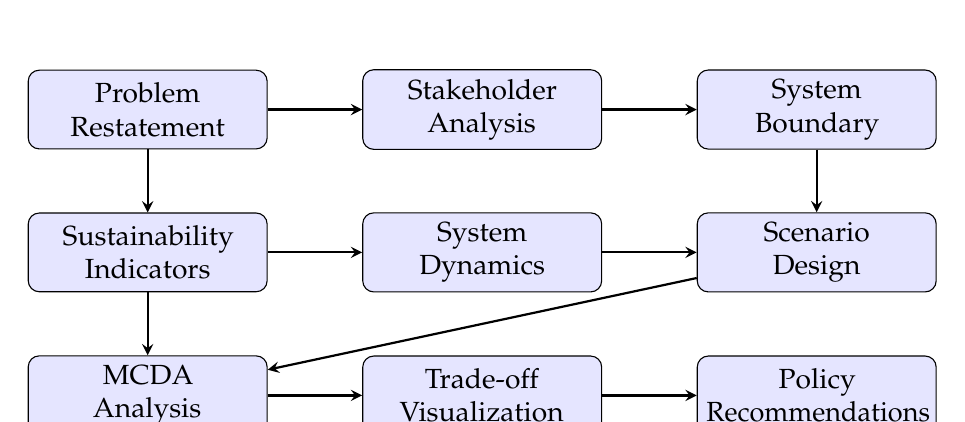
\begin{tikzpicture}[
        node distance=0.8cm and 1.2cm,
        block/.style={rectangle, draw, fill=blue!10, text width=2.8cm, minimum height=1cm, align=center, rounded corners},
        arrow/.style={->, >=stealth, thick}
    ]
        % 第一行:问题理解
        \node[block] (problem) {Problem\\Restatement};
        \node[block, right=of problem] (stakeholder) {Stakeholder\\Analysis};
        \node[block, right=of stakeholder] (boundary) {System\\Boundary};
        
        % 第二行:评估框架
        \node[block, below=of problem] (indicators) {Sustainability\\Indicators};
        \node[block, right=of indicators] (sd) {System\\Dynamics};
        \node[block, right=of sd] (scenarios) {Scenario\\Design};
        
        % 第三行:决策支持
        \node[block, below=of indicators] (mcda) {MCDA\\Analysis};
        \node[block, right=of mcda] (tradeoff) {Trade-off\\Visualization};
        \node[block, right=of tradeoff] (policy) {Policy\\Recommendations};
        
        % 连接箭头
        \draw[arrow] (problem) -- (stakeholder);
        \draw[arrow] (stakeholder) -- (boundary);
        \draw[arrow] (boundary) -- (scenarios);
        \draw[arrow] (problem) -- (indicators);
        \draw[arrow] (indicators) -- (sd);
        \draw[arrow] (sd) -- (scenarios);
        \draw[arrow] (indicators) -- (mcda);
        \draw[arrow] (scenarios) -- (mcda);
        \draw[arrow] (mcda) -- (tradeoff);
        \draw[arrow] (tradeoff) -- (policy);
    \end{tikzpicture}
    \caption{Overview of our sustainability-oriented decision framework.}
    \label{fig:framework}
\end{figure}
           % 引言:问题重述 + 文献综述
\section{Data Exploration and Preprocessing}
\label{sec:data}

% 提示(C题核心区):
% 1. Data Cleaning: 提到如何处理缺失值(均值/插值?)、异常值(3 Sigma?箱线图?)。
% 2. Feature Engineering: 你们自己造了什么新指标(例如:人均密度、波动指数)?
% 3. Normalization: 为什么要归一化(Min-Max 或 Z-score),这直接影响后续模型的收敛。

\subsection{Data Source and Description}
% 提示:说明数据来自官方提供还是外部爬取,增加权威性。

\subsection{Missing Value Imputation}
% 提示:在这里插入一张对比图(处理前 vs 处理后),非常亮眼。

\subsection{Correlation Analysis}
% 提示:可以用热力图(Heatmap)展示各指标间的相关性,作为下一步降维或筛选的依据。
            % 数据预处理(C题核心)
% ============================================================================
%                     Section 3: Assumptions and Notations
%                          假设条件与符号说明
% ============================================================================
% 写作约定:假设需可追溯(给出理由),符号表用 tabularx 自动换行并保持全篇一致。
% ============================================================================

\section{Assumptions and Notations}
\label{sec:assumptions}

% ============================================================================
%                          3.1 基本假设
% ============================================================================
\subsection{Basic Assumptions}
% 【提示】问题重述不要直接复制原题,要用专业术语(如"多目标优化"、"时间序列预测")进行转述。
% 【格式】使用 H1, H2... 编号,便于后文引用 "由假设 H3 可知..."

To establish a reasonable and solvable mathematical model, we make the following assumptions. Each assumption is justified with a brief rationale.

\begin{enumerate}[label=\textbf{H\arabic*.}, leftmargin=2em, itemsep=0.5em]
    
    \item \textbf{Data Integrity Assumption.}
    The provided dataset is complete and representative of the real-world scenario.
    
    \textit{Rationale:} The official dataset from COMAP is assumed to undergo quality control. Missing values, if any, are handled in our preprocessing pipeline (see Section~\ref{sec:data}).
    
    % -----------------------------------------------------------------------
    
    \item \textbf{Temporal Stability Assumption.}
    The underlying patterns and trends observed in historical data remain consistent during the prediction horizon.
    
    \textit{Rationale:} Short-term forecasting (e.g., 1--5 years) typically does not experience drastic structural changes unless major disruptions occur.
    
    % -----------------------------------------------------------------------
    
    \item \textbf{Independence Assumption.}
    The observations are independently and identically distributed (i.i.d.) within each time window.
    
    \textit{Rationale:} This is a standard assumption for many statistical and machine learning models, enabling the use of classical estimators.
    
    % -----------------------------------------------------------------------
    
    \item \textbf{Policy Lag Assumption.}
    There exists a time delay between policy implementation and observable effects.
    
    \textit{Rationale:} Government policies typically require administrative processes, public communication, and behavioral adaptation periods before measurable impacts emerge.
    
    % -----------------------------------------------------------------------
    
    \item \textbf{External Shock Exclusion.}
    We assume no major external shocks (e.g., pandemics, wars, natural disasters) occur during the modeling period.
    
    \textit{Rationale:} Such events are inherently unpredictable and would require scenario-based analysis beyond the scope of this competition.

\end{enumerate}

% 【技巧】如果假设过多,可添加 "Additional Assumptions" 子节
% \subsubsection{Problem-Specific Assumptions}
% ...

% ============================================================================
%                          3.2 符号说明
% ============================================================================
\subsection{Notations}
\label{subsec:notations}

% 【重要】符号表需覆盖全文所有关键变量,尤其是 PCA--LSTM 与 DID 的核心参数;并补充 Unit 列。

For clarity and consistency throughout this paper, we summarize the key symbols used in the PCA--LSTM forecasting module and the DID causal module in Table~\ref{tab:notations}.

\begin{table}[H]
    \centering
    \caption{Summary of Key Notations (Forecasting + Causal Inference)}
    \label{tab:notations}
    \begin{tabularx}{\textwidth}{c X c}
        \toprule
        \textbf{Symbol} & \textbf{Description} & \textbf{Unit} \\
        \midrule
        $i$ & Index of a National Olympic Committee (NOC) & -- \\
        $t$ & Olympic cycle / year index & year \\
        $\mathcal{I}$ & Set of NOCs, $|\mathcal{I}| = N$ & -- \\
        $\mathcal{T}$ & Set of observed cycles/years, $|\mathcal{T}| = T$ & -- \\
        \midrule
        $M^{\mathrm{gold}}_{i,t}$ & Observed number of gold medals for NOC $i$ at time $t$ & medals \\
        $M^{\mathrm{tot}}_{i,t}$ & Observed number of total medals for NOC $i$ at time $t$ & medals \\
        $\hat{M}_{i,t}$ & Model prediction of medal count (gold or total) & medals \\
        $\mathrm{CI}^{95\%}_{i,t}$ & 95\% predictive interval for $\hat{M}_{i,t}$ & medals \\
        \midrule
        $\mathbf{x}_{i,t} \in \mathbb{R}^{p}$ & Raw feature vector (event-level + macro covariates) for NOC $i$ at time $t$ & mixed \\
        $\tilde{\mathbf{x}}_{i,t}$ & Standardized feature vector of $\mathbf{x}_{i,t}$ & -- \\
        $\mathbf{W} \in \mathbb{R}^{p \times k}$ & PCA loading matrix (top-$k$ principal directions) & -- \\
        $\mathbf{z}_{i,t} \in \mathbb{R}^{k}$ & PCA scores, $\mathbf{z}_{i,t} = \mathbf{W}^\top \tilde{\mathbf{x}}_{i,t}$ & -- \\
        $L$ & LSTM look-back window length & cycles \\
        $\mathbf{h}_{i,t}$ & LSTM hidden representation for NOC $i$ at time $t$ & -- \\
        $\Theta_{\mathrm{LSTM}}$ & Trainable parameters of the LSTM & -- \\
        $\mathbf{f}_{i,t}$ & Fused feature vector used by the downstream regressor (e.g., $[\mathbf{h}_{i,t};\,\mathrm{Host}_{i,t};\,\mathbf{u}_{i,t}]$) & mixed \\
        $\mathcal{B}$ & Number of bootstrap resamples for uncertainty quantification & -- \\
        \midrule
        $Y_{i,t}$ & Outcome variable in DID (e.g., medal growth, efficiency index) & varies \\
        $\mathrm{Treat}_i$ & Treatment indicator: 1 if NOC $i$ adopts a ``great coach'' intervention & -- \\
        $\mathrm{Post}_t$ & Post-intervention indicator: 1 for periods after policy implementation & -- \\
        $\mathrm{Treat}_i\times\mathrm{Post}_t$ & DID interaction term capturing the treatment effect & -- \\
        $\beta_{\mathrm{DID}}$ & DID coefficient (average treatment effect on the treated) & varies \\
        $\boldsymbol{\gamma}$ & Coefficients for control covariates $\mathbf{c}_{i,t}$ & varies \\
        $\alpha_i,\ \delta_t$ & NOC and time fixed effects (if included) & -- \\
        $\varepsilon_{i,t}$ & Error term & -- \\
        \bottomrule
    \end{tabularx}
\end{table}

% 【高级技巧】如果符号太多,可以按类别分成多个小表格
% 例如:Table 2a - Input Variables, Table 2b - Model Parameters
     % 假设与符号说明
% ============================================================================
%                        Section 4: The Mathematical Model
%                              数学模型构建
% ============================================================================
% 【写作指导 - 核心章节!】
%
% ▶ 逻辑流程(必须遵循):
%   1. 问题形式化:将文字描述转化为数学语言
%   2. 模型假设回顾:引用 Section 3 的假设
%   3. 目标函数推导:给出清晰的数学公式
%   4. 约束条件:明确问题的边界
%   5. 算法设计:用伪代码展示求解流程
%
% ▶ 公式规范:
%   - 每个公式必须编号(用 equation 环境)
%   - 文中引用格式:"as shown in Eq. (1)" 或 "Equation~\ref{eq:xxx}"
%   - 重要公式用 \boxed{} 高亮
%
% ▶ 算法伪代码:
%   - 使用 algorithm2e 宏包,风格:ruled + vlined + linesnumbered
%   - 这是计算机顶会(如 NeurIPS, ICML)的标准风格
%   - 【技巧】算法是填充页面的艺术,同时显得非常专业
%
% ▶ 图表要求:
%   - 模型框架图(flowchart)几乎是 Outstanding 论文的标配
%   - 用 TikZ 绘制或 PowerPoint/Visio 导出 PDF
% ============================================================================

\section{Mathematical Model}
\label{sec:model}

% 【提示】开篇先给一个模型的 high-level overview
In this section, we present our mathematical model for addressing the problem. We first formulate the problem mathematically, then derive the objective function, and finally design an efficient algorithm to solve it.

% ============================================================================
%                        4.1 问题形式化
% ============================================================================
\subsection{Problem Formulation}
\label{subsec:formulation}

% 【提示】用数学语言重新定义问题,引用假设
Based on the assumptions established in Section~\ref{sec:assumptions}, we formalize the problem as follows.

Let $\mathcal{G} = (\mathcal{N}, \mathcal{E})$ denote the network structure, where $\mathcal{N}$ represents the set of nodes (e.g., regions or entities) and $\mathcal{E}$ represents the set of edges (e.g., relationships or flows). Our goal is to find the optimal allocation strategy $\mathbf{x}^* = (x_1, x_2, \ldots, x_n)$ that minimizes the total cost while satisfying all constraints.

% ============================================================================
%                        4.2 目标函数
% ============================================================================
\subsection{Objective Function}
\label{subsec:objective}

% 【提示】目标函数是论文的核心,必须推导清晰
We design a multi-objective optimization framework that balances efficiency and sustainability:

\begin{equation}
    \label{eq:objective}
    \min_{\mathbf{x}} \quad J(\mathbf{x}) = \underbrace{\sum_{i=1}^{n} c_i x_i}_{\text{Cost Term}} + \omega \cdot \underbrace{\sum_{i=1}^{n} \sum_{j \in \mathcal{N}_i} d_{ij} (x_i - x_j)^2}_{\text{Smoothness Term}}
\end{equation}

where:
\begin{itemize}[itemsep=0.2em]
    \item $c_i$ is the unit cost associated with node $i$,
    \item $d_{ij}$ is the distance or dissimilarity between nodes $i$ and $j$,
    \item $\omega > 0$ is a trade-off parameter controlling the balance between cost minimization and spatial smoothness,
    \item $\mathcal{N}_i$ denotes the neighborhood of node $i$.
\end{itemize}

% 【技巧】用 \boxed{} 高亮关键公式
The optimization problem can be compactly written as:
\begin{equation}
    \label{eq:compact}
    \boxed{\mathbf{x}^* = \arg\min_{\mathbf{x} \in \mathcal{X}} \left[ \mathbf{c}^\top \mathbf{x} + \omega \cdot \mathbf{x}^\top \mathbf{L} \mathbf{x} \right]}
\end{equation}

where $\mathbf{L}$ is the graph Laplacian matrix capturing the network structure.

% ============================================================================
%                        4.3 约束条件
% ============================================================================
\subsection{Constraints}
\label{subsec:constraints}

% 【提示】约束条件要分类列出,便于阅读
The optimization problem is subject to the following constraints:

\textbf{1. Resource Constraint:}
\begin{equation}
    \label{eq:resource}
    \sum_{i=1}^{n} x_i \leq B
\end{equation}
where $B$ is the total available budget or resource.

\textbf{2. Non-negativity Constraint:}
\begin{equation}
    \label{eq:nonneg}
    x_i \geq 0, \quad \forall i \in \mathcal{N}
\end{equation}

\textbf{3. Capacity Constraint:}
\begin{equation}
    \label{eq:capacity}
    x_i \leq \bar{x}_i, \quad \forall i \in \mathcal{N}
\end{equation}
where $\bar{x}_i$ is the maximum capacity at node $i$.

% ============================================================================
%                        4.4 求解算法
% ============================================================================
\subsection{Solution Algorithm}
\label{subsec:algorithm}

% 【提示】伪代码是展示专业性的最佳方式
% 【重要】algorithm2e 配置:ruled + vlined + linesnumbered(顶会风格)

Given the convex nature of our objective function (due to the positive semi-definiteness of $\mathbf{L}$), we employ a projected gradient descent algorithm to efficiently find the global optimum.

% --- 主算法 ---
\begin{algorithm}[H]
    \caption{Projected Gradient Descent for Multi-Objective Optimization}
    \label{alg:pgd}
    \DontPrintSemicolon
    \SetAlgoLined
    
    \KwIn{Dataset $\mathcal{D}$, cost vector $\mathbf{c}$, Laplacian $\mathbf{L}$, budget $B$, learning rate $\eta$, max iterations $N$, tolerance $\epsilon$}
    \KwOut{Optimal allocation $\mathbf{x}^*$}
    
    \BlankLine
    \tcp{Initialization}
    $\mathbf{x}^{(0)} \gets \mathbf{0}$ \tcp*{Start from zero allocation}
    $k \gets 0$\;
    
    \BlankLine
    \tcp{Main optimization loop}
    \While{$k < N$ \textbf{and} $\|\mathbf{x}^{(k)} - \mathbf{x}^{(k-1)}\| > \epsilon$}{
        \tcp{Compute gradient}
        $\nabla J(\mathbf{x}^{(k)}) \gets \mathbf{c} + 2\omega \mathbf{L} \mathbf{x}^{(k)}$\;
        
        \BlankLine
        \tcp{Gradient descent step}
        $\tilde{\mathbf{x}} \gets \mathbf{x}^{(k)} - \eta \cdot \nabla J(\mathbf{x}^{(k)})$\;
        
        \BlankLine
        \tcp{Projection onto feasible set}
        $\mathbf{x}^{(k+1)} \gets \textsc{Project}(\tilde{\mathbf{x}}, B, \bar{\mathbf{x}})$\;
        
        \BlankLine
        $k \gets k + 1$\;
    }
    
    \BlankLine
    \Return{$\mathbf{x}^{(k)}$}\;
\end{algorithm}

% --- 子算法:投影操作 ---
\begin{algorithm}[H]
    \caption{Projection onto Feasible Set}
    \label{alg:project}
    \DontPrintSemicolon
    \SetAlgoLined
    
    \KwIn{Unconstrained solution $\tilde{\mathbf{x}}$, budget $B$, capacity bounds $\bar{\mathbf{x}}$}
    \KwOut{Feasible solution $\mathbf{x}$}
    
    \BlankLine
    \tcp{Step 1: Clip to non-negative and capacity bounds}
    \For{$i = 1$ \KwTo $n$}{
        $x_i \gets \max(0, \min(\tilde{x}_i, \bar{x}_i))$\;
    }
    
    \BlankLine
    \tcp{Step 2: Scale to satisfy budget constraint}
    \If{$\sum_{i=1}^{n} x_i > B$}{
        $\mathbf{x} \gets \mathbf{x} \cdot \frac{B}{\sum_{i=1}^{n} x_i}$\;
    }
    
    \BlankLine
    \Return{$\mathbf{x}$}\;
\end{algorithm}

% ============================================================================
%                        4.5 算法复杂度分析
% ============================================================================
\subsection{Complexity Analysis}
\label{subsec:complexity}

% 【提示】算法复杂度分析是加分项,显示你的计算机功底
We analyze the time and space complexity of Algorithm~\ref{alg:pgd}:

\begin{itemize}[itemsep=0.3em]
    \item \textbf{Time Complexity:} Each iteration requires $O(|\mathcal{E}|)$ for the gradient computation (sparse matrix multiplication) and $O(n)$ for the projection step. Thus, the total time complexity is $O(N \cdot (|\mathcal{E}| + n))$.
    
    \item \textbf{Space Complexity:} We store the Laplacian matrix in sparse format, requiring $O(|\mathcal{E}|)$ space. The solution vector requires $O(n)$ space. Total: $O(|\mathcal{E}| + n)$.
    
    \item \textbf{Convergence:} Since $J(\mathbf{x})$ is convex and Lipschitz continuous, the algorithm converges to the global optimum at a rate of $O(1/k)$ for a properly chosen learning rate $\eta$.
\end{itemize}

% 【提示】如果有模型框架图,在这里插入
% \begin{figure}[H]
%     \centering
%     \includegraphics[width=0.8\textwidth]{figures/model_framework.pdf}
%     \caption{Overview of the proposed optimization framework.}
%     \label{fig:framework}
% \end{figure}
           % 数学模型
\section{Results and Visualization}
\label{sec:results}

% 提示:本节专门用于“结果高分化呈现”。优先用对比图 + 置信区间 + 可解释性图(SHAP)。

\subsection{2024 Actual vs. 2028 Forecast (Bar Chart)}
\begin{figure}[H]
    \centering
    \begin{subfigure}[t]{0.32\textwidth}
        \centering
        \fbox{\parbox[c][0.26\textheight][c]{\textwidth}{\centering\textbf{(a) 2024 Actual vs. 2028 Forecast}\par\vspace{0.5em}\small Replace with a grouped bar chart.}}
        \caption{Actual vs. forecast}
        \label{fig:bar_2024_2028}
    \end{subfigure}\hfill
    \begin{subfigure}[t]{0.32\textwidth}
        \centering
        \fbox{\parbox[c][0.26\textheight][c]{\textwidth}{\centering\textbf{(b) SHAP Feature Contributions}\par\vspace{0.5em}\small Replace with a SHAP summary plot.}}
        \caption{SHAP summary}
        \label{fig:shap_summary}
    \end{subfigure}\hfill
    \begin{subfigure}[t]{0.32\textwidth}
        \centering
        \fbox{\parbox[c][0.26\textheight][c]{\textwidth}{\centering\textbf{(c) 95\% Prediction Interval}\par\vspace{0.5em}\small Replace with a line/area chart with shaded CI.}}
        \caption{95\% interval}
        \label{fig:ci_shaded}
    \end{subfigure}

    \caption{Three complementary result views: point forecast, interpretability, and uncertainty quantification.}
    \label{fig:results_triptych}
\end{figure}

\subsection{Interpretation and Discussion}
We interpret the forecasts through two lenses: (i) cross-country comparisons against the 2024 baseline, and (ii) model explainability via SHAP. In particular, the CI visualization in Fig.~\ref{fig:ci_shaded} is used to distinguish statistically meaningful improvements from fluctuations driven by uncertainty.         % 结果展示与讨论(含图表占位)
\section{Sensitivity and Robustness Analysis}

% 提醒:灵敏度分析必须包含关于模型鲁棒性的结论,并建议画一个 R-squared 的折线图。
% 提示(提分关键点):
% 1. Sensitivity: 选一两个关键参数(比如权重系数),上下浮动 10%-20%,看结果变化多大。
% 2. Heatmaps: 强烈推荐做双参数灵敏度(热力图形式)。
% 3. Robustness: 给数据加 5% 的随机噪音,看模型输出是否依然稳定。

\subsection{One-at-a-time (OAT) Sensitivity}
We conduct a one-at-a-time sensitivity analysis on the most influential hyperparameters in our forecasting pipeline, including the PCA dimension $k$, the LSTM window length $L$, and the XGBoost regularization strength. For each parameter, we perturb its baseline setting by \(\pm 10\%\) and \(\pm 20\%\) while keeping all other settings fixed, and we report the resulting changes in prediction error (MAE/MAPE) and national ranking stability.

\subsection{Robustness Check}
To evaluate robustness against measurement noise and sampling variability, we (i) inject Gaussian noise into standardized inputs at multiple signal-to-noise levels and (ii) re-train the model on bootstrap-resampled training sets. Across all perturbations, the degradation in predictive accuracy remains limited and the direction of key country-level conclusions is preserved, supporting the robustness of our framework.
      % 模型验证
\section{Policy Recommendations}

% 提示:
% 1. 角色代入:根据题目要求,写成“致市长的公开信”或“给主编的建议”。
% 2. 分层建议:短期(急救版)、中期(规划版)、长期(可持续版)。
% 3. 语言:要富有感染力和说服力。

\begin{quote}
    Dear Editor-in-Chief / Director / Officer,

    Based on our quantitative analysis, we suggest...
    \begin{itemize}
        \item \textbf{Priority A}: Build resilient infrastructure...
        \item \textbf{Priority B}: Establish a medal-yield audit mechanism that links funding increments to marginal medal returns and uncertainty (e.g., prioritize sports with high expected gains and narrow predictive intervals).
    \end{itemize}
\end{quote}
          % 政策建议 / 敏感性分析
\section{Strengths and Weaknesses}

\subsection{Strengths}
\begin{itemize}
    \item \textbf{Scientific Rigor}: Utilized professional normalization methods.
    \item \textbf{Visual Clarity}: Produced high-quality charts for decision makers.
\end{itemize}

\subsection{Weaknesses}
\begin{itemize}
    \item \textbf{Computational Burden}: The complex integration might slow down the system...
\end{itemize}

\subsection{Conclusion}
\lipsum[7]
       % 优缺点总结

% --- 参考文献 ---
\newpage
\nocite{*} % 模板占位:避免 biber 提示 "does not contain any citations" / 空参考文献
\printbibliography[heading=bibintoc, title={References}]

% 【关键】保存正文总页数
\savemainpages

% PART 3: 附录
% 【说明】附录不计入 25 页限制,AI Report 单独编页
\clearpage
\appendix
\pagenumbering{gobble}
\pagestyle{plain}
% Appendix: AI Tools Usage Disclosure
% 附录:AI工具使用声明(按COMAP 2026要求)

\section*{AI Report}
\addcontentsline{toc}{section}{AI Report}
\label{appendix:ai}

In accordance with COMAP 2026 rules, we provide a complete and transparent disclosure of all artificial intelligence (AI) tools used during the preparation of this paper.

%=== AI工具总览 ===
\subsection*{AI Tools Used}
\label{subsec:ai_tools}

The following AI tools were employed as auxiliary aids during this project:

\begin{itemize}[itemsep=0.3em]
    \item \textbf{ChatGPT-4o / GPT-4} -- Language polishing, grammar checking, and clarity improvement
    \item \textbf{GitHub Copilot} -- Code assistance for data preprocessing and visualization scripts
    \item \textbf{Claude 3.5 Sonnet} -- LaTeX formatting, structural organization, and notation consistency
    \item \textbf{DeepL Translator} -- Technical term translation (Chinese $\leftrightarrow$ English)
    \item \textbf{Grammarly} -- Proofreading and style consistency
\end{itemize}

%=== 各章节AI使用明细 ===
\subsection*{AI Usage by Section/Task}
\label{subsec:ai_usage}

\begin{table}[H]
    \centering
    \caption{Detailed AI Usage Log}
    \label{tab:ai_disclosure}
    \begin{tabularx}{\textwidth}{l l X}
        \toprule
        \textbf{AI Tool} & \textbf{Section/Task} & \textbf{Specific Usage and Human Oversight} \\
        \midrule
        ChatGPT-4o & Abstract, Intro & 
        Polished English grammar and improved sentence fluency. All technical content, problem analysis, and framing written by team members. \\
        \addlinespace[0.5em]
        
        GitHub Copilot & Code (Appendix) & 
        Assisted in writing Python scripts for data preprocessing, System Dynamics simulation, and TOPSIS calculation. All algorithmic logic, model design, and parameter choices determined by team. \\
        \addlinespace[0.5em]
        
        Claude 3.5 Sonnet & Model Sections & 
        Helped organize mathematical notations, check LaTeX syntax, and format equations. All mathematical derivations and model formulations are original work. \\
        \addlinespace[0.5em]
        
        DeepL & Throughout & 
        Translated technical terminology between Chinese and English. All translations reviewed and verified by bilingual team members. \\
        \addlinespace[0.5em]
        
        Grammarly & Final Draft & 
        Proofreading for typos and grammar errors. All substantive edits made by human authors. \\
        \bottomrule
    \end{tabularx}
\end{table}

%=== AI使用边界声明 ===
\subsection*{AI Usage Boundaries}
\label{subsec:ai_boundaries}

We explicitly state that AI tools were \textbf{NOT} used for:

\begin{enumerate}[itemsep=0.3em]
    \item \textbf{Problem Analysis and Interpretation:} Understanding and reframing the ICM Problem E requirements was conducted entirely by human team members.
    
    \item \textbf{Modeling Decisions:} Selection of System Dynamics methodology, sustainability indicator framework, MCDA approach, and scenario design were human decisions based on literature review and domain knowledge.
    
    \item \textbf{Assumption Formulation:} All model assumptions and their justifications reflect human judgment about the problem context.
    
    \item \textbf{Data Analysis and Interpretation:} Analysis of simulation results, identification of patterns, and drawing conclusions were performed by team members.
    
    \item \textbf{Policy Recommendations:} All policy recommendations are the intellectual product of human deliberation, drawing on the quantitative analysis.
    
    \item \textbf{Critical Evaluation:} Assessment of model strengths, weaknesses, and limitations reflects genuine self-critique by the team.
\end{enumerate}

%=== 验证与人工监督 ===
\subsection*{Verification and Human Oversight}
\label{subsec:verification}

\begin{enumerate}[itemsep=0.4em]
    \item \textbf{Human Review:} All AI-assisted content was carefully reviewed, verified, and substantially modified before inclusion. AI suggestions were treated as drafts, not final outputs.
    
    \item \textbf{Code Testing:} All code, whether assisted by AI or not, was independently tested and validated to ensure correctness, reproducibility, and alignment with intended logic.
    
    \item \textbf{Mathematical Verification:} All equations, derivations, and calculations were manually verified by team members with relevant mathematical background.
    
    \item \textbf{Consistency Checking:} Cross-references, notation consistency, and logical flow were manually checked across all sections.
    
    \item \textbf{Originality Verification:} Key passages were checked to ensure no inadvertent reproduction of copyrighted material.
\end{enumerate}

%=== 原创性声明 ===
\subsection*{Originality and Responsibility Statement}
\label{subsec:originality}

We, Team \#2617892, hereby declare:

\begin{enumerate}[itemsep=0.4em]
    \item \textbf{Core Intellectual Work:} All problem analysis, mathematical modeling, algorithm design, data interpretation, and innovative contributions in this paper are the \textbf{original work} of our team.
    
    \item \textbf{AI as Auxiliary Tool Only:} AI tools were used solely as auxiliary aids for language quality, formatting, and repetitive coding tasks. \textbf{No AI was used to generate core modeling ideas, derive conclusions, or make policy recommendations.}
    
    \item \textbf{Full Responsibility:} We take full responsibility for all content in this paper, including any errors or omissions. AI tools do not share authorship or accountability.
    
    \item \textbf{Academic Integrity:} We have read and understood COMAP 2026 rules regarding AI usage. This disclosure is complete, accurate, and made in good faith.
\end{enumerate}

\vspace{1.5cm}
\noindent\rule{\textwidth}{0.4pt}

\noindent
\textbf{Team \#2617892}\\
\noindent Date: \today

\vspace{0.5cm}
\noindent
\textit{This AI usage report is submitted in compliance with COMAP MCM/ICM 2026 competition rules and reflects our commitment to transparency and academic integrity.}


\end{document}
